\documentclass{clv3}
\usepackage[UTF8]{ctex}
\usepackage{hyperref}
\usepackage{xcolor}
\usepackage{enumerate}
\usepackage{graphicx}
\usepackage{amsmath}
\definecolor{darkblue}{rgb}{0, 0, 0.5}
\hypersetup{colorlinks=true,citecolor=darkblue, linkcolor=darkblue, urlcolor=darkblue}

\bibliographystyle{compling}


\issue{1}{1}{2019}


\begin{document}

\title{情感分析综述} % 修改此处

\author{李开运} % 修改此处
\affil{中国科学院大学} % 修改此处


\maketitle

\begin{abstract} % 修改此处
文本情感分析:又称意见挖掘、倾向性分析等。简而言之,是对带有情感色彩的主观性文本进行分析、处理、归纳和推理的过程。随着信息技术快速发展,互联网上产生了大量的用户参与的、对于诸如人物、事件、产品等有价值的评论信息。这些评论信息表达了人们的各种上情感色彩和情感倾向性。作为自然语言处理领域的一个重要分支,情感分析在理论方面有着较高的研究意义。本文首先对文本情感分析工作的研究背景和意义进行了介绍,然后对文本情感分析的理论与研究方法进行了总结,最后探讨了情感分析技术未来的发展方向。
\end{abstract}

\section{引言} 
根据中国互联网网络信息中心(CNNIC)的统计,目前我国已有8.02亿的网民,互联网普及率为57.7\%。信息技术水平的不断提高和互联网产业的快速发展,也为人们提供了各种平台,如社交网络、电商平台、政务网站、生活服务类APP等。网络用户之间的交互关系不断得到发展体现,用户不再是单方面地从网络中获取信息,更成为了网络中内容的创造者。用户生成的大量内容中文本信息占很大比例,这些文本内容以可以细分客观文本和主观文本。而主观性文本中所蕴含的用户情感态度信息具有重要价值。

自然语言处理(NLP)领域的一个重要的研究方向就是情感分析。在2003年,Nasukawa\cite{sentiment}等人就提出了情感分析的概念,并描述了情感分析的任务内容和工作难点,引起了学术界人士的广泛关注。情感分析工作,也称为意见和评论挖掘,是对带有情感倾向的主观文本进行分析,从中提取情感或观点的过程。文本情感分析是一个涉及多个领域的综合性研究学科。对情感分析任务而言,文本内容的组成部分主要有意见的持有人、评价对象、情感类别等。按照处理文本的粒度不同,情感分析大致可分为词语级、句子级、篇章级三个研究层次。根据分类的目的不同,情感分析工作的子任务有主的分析和情感态度的分类两种。对于不同的文本情感分析任务也可以采用不同的情感类别体系。众多的情感分析技术中,大致可以分为2个重要步骤:1)情感信息抽取;2)情感分类。
\section{情感信息抽取}
情感分析的最底层的任务,它旨在抽取情感评论文本中有意义的信息单元,情感信息抽取可提炼出对情感分析有贡献的词或短语元素,其结果对特征降维、提高系统性能有重要作用,。情感信息抽取包括三个方面:
\begin{enumerate}[(1)]
	\item 评论词语的抽取和判别
	\item 评价对象的抽取
	\item 观点持有者的抽取
\end{enumerate}
常用的统计分析方法有基于信息增益、互信息、期望交差熵、词频、文档频次等
\subsection{基于文档频率的特征提取法}
文档频率(DF)是指出现某个特征项的文档的频率。基于文档频率的特征提取法通常的做法是:从训练语料中统计出包含某个特征的文档的频率(个数),然后根据设定的阈值,当该特征项的DF值小于某个阈值时,从特征空间中去掉该特征项,因为该特征项使文档出现的频率太低,没有代表性;当该特征项的DF值大于另外一个阈值时,从特征空间中也去掉该特征项,因为该特征项使文档出现的频率太高,没有区分度。
\subsection{信息增益法}
信息增益(IG)法依据某特征项$t_i$为整个分类所能提供的信息量多少来衡量该特征项的重要程度,从而决定对该特征项的取舍。某个特征项$t_i$的信息增益是指有该特征或没有该特征时,为整个分类所能提供的信息量的差别,其中,信息量的多少由熵来衡量。因此,信息增益即不考虑任何特征时文档的熵和考虑该特征后文档的熵的差值:
\begin{equation}
	\begin{aligned}
		\mathrm{Gain}(t_i)&=\mathrm{Entropy}(S)-\mathrm{Expected\ Entropy}(S_{t_i})\\
		&=\left\{-\sum_{j=1}^{M}P(C_j)\times \log P(C_j) \right\}-\left\{P(t_i)\times \left[-\sum_{j=1}^{M}P(C_j|t_i)\times \log P(C_j|t_i) \right] \right.\\
		&\ \left. +P(\bar{t}_i)\times \left[-\sum_{j=1}^{M}P(C_j|\bar{t}_i)\times \log P(C_j|\bar{t}_i)\right]\right\}
	\end{aligned}
\end{equation}
\subsection{$\chi^2$统计量}
$\chi^2$统计量(CHI)衡量的是特征项$t_i$和类别$C_j$之间的相关程度,并假设$t_i$和$C_j$之间符合具有一阶自由度的$\chi^2$分布。特征对于某类的$\chi^2$统计值越高,它与该类之间的相关性越大,携带的类别信息也较多,反之则越少。特征项$t_i$对$C_j$的CHI值为
\begin{equation}
	\chi^2(t_i,C_j)=\frac{N\times (A\times D-C\times B)^2}{(A+C)\times (B+D)\times (A+B)\times (C+D)}
\end{equation}
\subsection{互信息法}
互信息(MI)法的基本思想是:互信息越大,特征$t_i$和类别$C_j$共现的程度越大。
\begin{equation}
	\begin{aligned}
		I(t_i,C_j)&=\log \frac{P(t_i,C_j)}{P(t_i)P(C_j)}\\
		&=\log \frac{P(t_i|C_j)}{P(t_i)}\\
		&\approx \frac{A\times N}{(A+C)\times (A+B)}
	\end{aligned}
\end{equation}
\section{情感分类} 
情感分类首要的是对文本的主客观性进行甄别,在新闻,个人博客,以及电影评论中都会涉及到一些客观事物描述,比如电影评论中涉及到对电影中的剧透,这些客观的描述潜在会包含情感词,而不能作为用户的情感计算。主、各观信息的分类可以参考如下两种方式:
\begin{enumerate}[(1)]
	\item 通过考察文本内容是否含有情感知识(具体表现为情感信息抽取的结果)来完成主客观信息分类。
	\item 将情感文本单元的主客观分类定义为一种二元分类任务,即对任意给定的情感文本单元,由分类器协助判断主客观性。这种方法的关键在于分类器和分类特征的选取。
\end{enumerate}

\section{情感分析技术介绍}
\subsection{传统的情感分析技术}
在传统的文本情感分析工作中,常用的方法主要可以分为两类:情感词典的分析方法和机器学习算法的分析方法。两种方法应用的技术不同,但都存在着一定的局限性。

\begin{figure}[htbp]
\begin{center}
	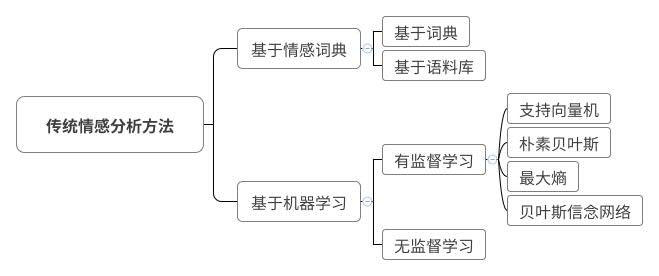
\includegraphics[width=\linewidth]{传统情感分析方法.jpg}
	\caption{something}\label{fig:1}
\end{center}
\end{figure}

情感词典是情感词汇的集合。情感词典主要包含不同情感色彩的词语,如积极、消极等,每个词语有对应的情感倾向值。使用这种方式,首先需要对被分析的文档中的情感词汇进行识别,然后将识别出的词语在情感词典中进行匹配比较工作。同时结合否定词、程度副词等信息,进行组合分析,依据设计的规则进行态度倾向值的计算,确定最终的情感倾向类别。由此可知使用情感词典方法的关键指出在于情感词典的构建和规则的制定。情感词典是判断情感极性的主要依据,同时根据语言学句法结构,设计相应的规则,比如and,so等连接后面的句子情感极性多与前方文相似。使用情感词典的文本情感分析方法的性能在很大程度上取决于词典的质量和判断规则是否有效。因此,情感词典的构建工作也受到也领域内相关研究人员的关注。构建情感词典的方法可以分为三类:基于手工方法、基于词典和基于语料的方法。但随着互联网的发展,信息量剧增,也出现了很多新兴词汇,对情感词典的构建维护工作生成了巨大的挑战,单纯使用情感词典的方法完成情感分析工作也就存在着很大的局限性。

基于机器学习的分析方法在近年来也得到了广泛的关注,这种使用统计学习的分析方法不再依赖情感词典,而是根据各种机器学习算法对文本进行统计分析。机器学习有两种上主要的方式:有监督学习和无监督学习。在2002年,\cite{pang}等人最早使用了机器学习算法进行情感分析的研究,在论文中比较分析了支持向量机、朴素贝叶斯、最大熵等算法,取得也良好的分类效果。在主客观分析上,\cite{mali}等人结合了情感词典与机器学习方法,使用了情感特征完成分析工作。在基于机器学习的方法中,最终结果的准确度在很大程度上取决于特征提取结果的质量,这具有一定的局限性。

部分情感分类的研究工作将基于词典的方法和基于机器学习的方法相融合。这类混合方法的思路主要分为2种:1)将“词典+规则”视作简单的分类器,然后融合多种不同分类器进行情感分类;2)将词典信息作为一种特征与现有特征(如句法特征、POS特征等)进行组合,然后选择最优的特征组合进行情感分类。\cite{prabowo}提出了一种基于规则的分类器(rule-based classifier, RBC)和支持向量机分类器(SVM)混合的方法,解决文档级别的情感分类问题。\cite{fang}等人提出将词典信息融入到支持向量机分类器中,解决语句级别的情感分类问题。
综上,传统的文本情感分析方法已经获得了不错的效果,但仍然存在着一些问题:
\begin{enumerate}[(1)]
	\item 基于情感词典的分析方法很大程度上依赖于构建的情感词典的质量,而情感词典一般不能涵盖、细分不同领域的词语,在一些新兴词汇的构建上也存在着一定的缺陷,会影响基于情感的情感分析的性能。

	\item 基于机器学习的文本情感分析方法的性能取决于特征提取工作完成的质量。目前,在对训练以及测试数据进行描述时,典型常用的方法是将单个词汇作为特征,而语言学中,文本的上下文语境十分重要,机器学习的方法不能充分有效地利用上下文信息对语句进行建模,影响分类结果的准确性。

	\item 不同领域的文本数据之间差异较大,而传统的文本情感分析方法的泛化能力较差,对于不同领域的任务模型性能比较差
\end{enumerate}


\subsection{基于深度学习的情感分析技术}
2006年,\cite{hinton}等人提出了深度学习的概念。随着词向量技术的提出和深度学习理论的发展,神经网络模型也逐渐被应用到情感分析等NLP相关研究任务中。NLP任务有几个特点:首先,输入是一维线性序列;其次是不定长的;再次,单词或者子句的相对位置关系很重要,两个单词位置互换或能导致完全不同的意思;最后,句子中的长距离特征对于理解语义也非常关键。一个特征抽取器是否适配问题领域的特点,有时候决定了它的成败,而很多模型改进的方向,其实就是改造使得它更匹配领域问题的特性。

RNN自从引入NLP界后,很快就在NLP各种任务中被广泛使用。但是原始的RNN也存在问题,它采取线性序列结构不断从前往后收集输入信息,但这种线性序列结构在反向传播的时候存在优化困难问题,因为反向传播路径太长,容易导致严重的梯度消失或梯度爆炸问题。为也解决这个问题,后来引入了LSTM\cite{lstm}和GRU\cite{gru}模型,通过增加中间状态信息直接向后传播,以此缓解梯度消失问题,获得了很好的效果,于是很快LSTM和GRU成为RNN的标准模型。后来NLP又从图像领域借鉴并引入了attention机制,叠加网络把层做深,以及引入Encoder-Decoder框架,这些技术进展极大拓展了RNN的能力以及应用效果。

基于RNN模型的特征提取器有两个缺点:1)表达能力有限;2)不具备能力。基于此,经过特殊改造的CNN\cite{cnn}模型,以及最近流行起来的Transformer\cite{transfomer}慢慢动摇着基于RNN模型的特征提取器的地位。

从语义特征提取能力来说,目前实验支持如下结论:Transformer在这方面的能力非常显著地超过RNN和CNN,RNN和CNN两者能力差不太多。
从长距离特征捕获能力来说,实验支持如下结论:Transformer和RNN在这方面能力差不太多,而CNN则显著弱于前两者。
从任务综合特征抽取能力来说,Transformer综合能力要明显强于RNN和CNN,而RNN和CNN表现基本相当。

自从深度学习流行起来后,预训练过程就是做图像或者视频领域的一种比较常规的做法,有比较长的历史了,而且这种做法很有效,能明显促进应用的效果。预训练模型一般有两种使用方法。1)浅层加载的参数在训练任务过程中不动,一般叫做“Frozen”;2)底层网络参数在训练过程中随着训练的进程不断改变,这种一般叫做“Fine-Tuning”。NLP领域借鉴了这种思想。

一般NLP领域做预训练一般的选择是用语言模型任务来做。在传统的语言模型中,存在着维度灾难的问题,而且缺乏建模相似词语之间关系的能力,Bengio\cite{nnlm}通过使用三层的神经网络构建神经网络语言模型(Nerural Network Language Model, NNLM),并得到了词语的向量表示。NNLM关注的重点是语言模型,词向量是研究过程中的一个副产品。事实上,大部分情况下,词向量和语言模型都是捆绑在一起的,训练完成后两者同时得到。Mikolov将研究中心放在词向量的表示中提出了Word2Vec,其思想还要追溯到Hinton于1986年提出的分布式表示(引用:distributed-representations)。后来又出了Glove\cite{glove}。Word Embedding存在一个最大的问题是多义词问题。ELMO(Embedding from Language Models)\cite{elmo}提供了一种简洁优雅的解决方案。在此之前的Word Embedding本质上是个静态的方式。ENMO的本质思想是:我事先用语言模型学好一个单词的Word Enbedding,此时多义词无法区分,不过这没关系。在我实际使用Word Embedding 的时候,单词已经具备了特定的上下文了,这个时候我可以根据上下文单词的语义去调整单词的Word Embedding表示,这样经过调整后的Word Embedding更能表达在这个上下文中的具体含义,自然也就解决了多义词的问题了,所以ELMO本身是个根据当前上下文对Word Embedding动态调整的思路。
GTP\cite{gpt}是”Generative Pre-Training”的简称。与ELMO类似,主要不同在于两点:首先,特征抽取器不是用的RNN,而是用的Transformer;其次,GPT的预训练虽然仍然是以语言模型作为目标任务,但是采用的是单向的语言模型。GPT的效果是非常令人惊艳的。
Bert\cite{bert}采用和GPT完全相同的两阶段模型,首先是语言模型预训练;其次是使用Fine-Tuning模式解决下游任务。和GPT最主要不同在于在预训练阶段采用了类似ELMO的双向语言模型,当然另外一点是语言模型的数据规模要比GPT大。目前而言,Bert取得了最好的效果。
情感分析模型

神经网络模型的使用不可避免地要涉及词向量嵌入技术。\cite{giatsoglou}等人将Word2Vec提供的上下文敏感编码与词典提供的情感信息相结合。虽然词向量嵌入技术考虑了单词的上下文,但是忽略了整体文本的情感。\cite{liangbin}等人提出了多注意力卷积神经网络MATT-CNN改善了效果。
\cite{socher}等人在2011-2013年间的研究工作中提出了一系列基于递归神经网络(resursive neural network, RecNN)的分类模型来解决情感分类问题。\cite{kim}则使用卷积神经网络(convolutional neural network, CNN)来解决情感分类问题。\cite{kalchbrenner}等人提出了一种新颖的卷积神经网络模型,该模型特点在于采用了动态k-max池化(dynamic k-max pooling)操作和多层卷积神经网络层相结合的结构。不同于止述式作,有研究者提出使用序列模型如循环神经网络(recurrent neural network, RNN)来解决情感分类问题,例如文献\cite{sa-lstm}。Yanmei等人在文献\cite{rnn-cnn}中提出了结合卷积神经网络和递归神经网络的微博情感分析方法,该方法首先利用卷积神经网络CNN学习特征向量,然后再利用递归神经网络RNN训练分类器进行微博情感分析。

综上所述,相比于传统机器学习方法,深层神经网络的表达能力有了质的飞跃,并摆脱了特征工程的束缚。加上特征提取技术的提升,预训练模型的应用,使得深度学习方法成为当下最好的解决情感分析的方法。
\section{总结}
本文对情感分析技术进行了系统性归纳,并着重介绍了深度学习方法在情感分析中的最新研究进展。本节我们简要梳理传统情感分类方法的不足,并总结深度学习的要点和挑战。

传统情感分析方法中,基于词典的方法过于依赖情感词典的构建,而机器学习方法的关键在于特征设计。无论是生成情感词典还是设计分类特征,都要求相关人员具有丰富的领域知识。此外,传统机器学习方法中的分类特征一般只能针对特定问题,推广能力有限。相比而言,深度模型拥有更强大的表达能力,能够更好地学习从数据到情感语义的复杂映射函数。但是,深度模型的训练是关键挑战。一方面,由于文本数据分布与所要预测的情感语义之间没有很强的相关性,所以无监督预训练方法在情感分类问题上效果欠佳;另一方面,有监督训练方法需要大量有标注数据来训练深度模型,而获得大规模有标注评论语句需要耗费大量人力进行数据标注工作。因此基于弱监督的深度学习方法会是解决情感分析问题的新思路。
\starttwocolumn
\bibliographystyle{plain}
\bibliography{mypaper} % 修改"mypaper.bib"文件
\end{document}
